\section{Chapter 10}
\subsection{10.1}
For Exercises 4, 6 and 8, determine whether the graph shown has
directed or undirected edges, whether it has multiple edges,
and whether it has one or more loops. Use your answers to
determine the type of graph in Table 1 this graph is.
\begin{itemize}
      \item[4.] \text{} \\ %To get the top of graphic to align w/ top
            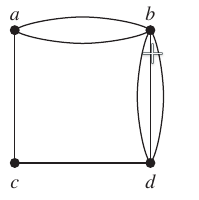
\includegraphics[scale = 0.7]{img/10_1_4_graph.png} \\
            \answer \\
            Undirected with multiple edges. So it's a multigraph.

      \item[6.] \text{} \\
            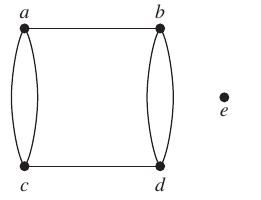
\includegraphics[scale = 0.7]{img/10_1_6_graph.png} a\\
            \answer\\
            Undirected with multiple edges. It's a multigraph.

      \item[8.] \text{} \\
            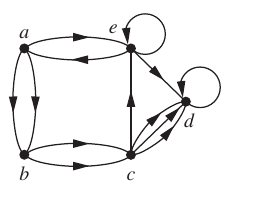
\includegraphics[scale = 0.7]{img/10_1_8_graph.png} \\
            \answer \\
            Directed with multiple edges and loops. It's a directed multigraph.

      \item[18.] Who can influence Fred and whom can Fred influence in
            the influence graph in Example 2? \\
            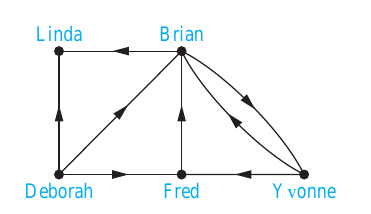
\includegraphics[scale = 0.7]{img/10_1_18_graph.png} \\
            \answer \\
            Fred can influence Brian, and he can be influenced by Yvonne and Deborah.
      \item[32.]  Which statements must be executed before $S_6$ is executed
            in the program in Example 8? (Use the precedence graph in Figure 10.)\\
            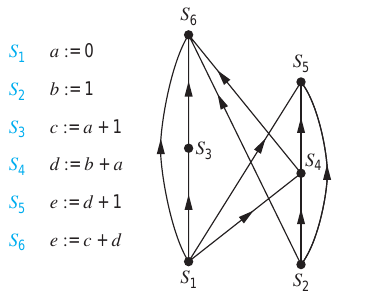
\includegraphics[scale = 0.7]{img/10_1_32_graph.png} \\
            \answer \\
            $S_1,\ S_2,\ S_3,\ S_4$
\end{itemize}

\subsection{10.2}
\begin{itemize}
      \item[6.] Show that the sum, over the set of people at a party, of
            the number of people a person has shaken hands with, is
            even. Assume that no one shakes his or her own hand. \\
            \answer \\
            The sum must be even becuase the total goes up by 2 each time someone shakes
            another person's hand because it goes up by one for each person. Therefore
            the final total must be even.

      \item[14.] What does the degree of a vertex in the Hollywood graph
            represent? What does the neighborhood of a vertex represent?
            What do the isolated and pendant vertices represent? \\
            \answer \\
            The degree represents the amount of actors that person has worked with.
            The neighborhood represents the set of specific actors they have worked
            with. The isolated vertices mean that the actor haven't worked with
            anyone. The pendant vertices represent the actors/actressses who have
            only done a movie with one other actor/actress.

      \item[20.]  Draw these graphs.
            \begin{enumerate}[a.]
                  \item $K_7$
                  \item $K_{1,8}$
                  \item $K_{4,4}$
                  \item $C_7$
                  \item $W_7$
                  \item $Q_4$
            \end{enumerate}
            \answer
            \begin{enumerate}[a.]
                  \item \text{}\\
                        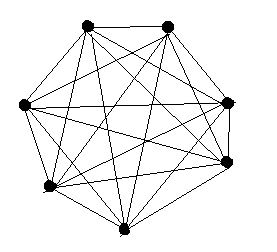
\includegraphics[scale=0.7]{img/10_2_20a_graph.png}
                  \item \text{}\\
                        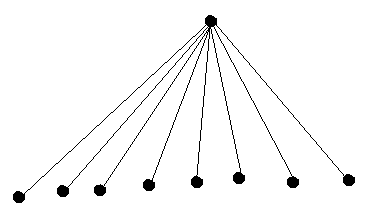
\includegraphics[scale=0.7]{img/10_2_20b_graph.png}
                  \item \text{}\\
                        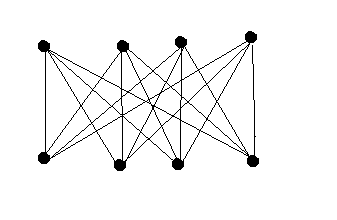
\includegraphics[scale=0.7]{img/10_2_20c_graph.png}
                  \item \text{}\\
                        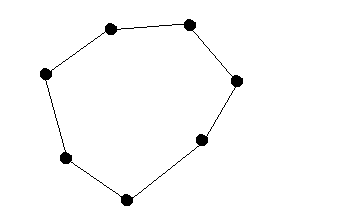
\includegraphics[scale=0.7]{img/10_2_20d_graph.png}
                  \item \text{}\\
                        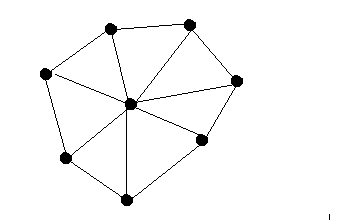
\includegraphics[scale=0.7]{img/10_2_20e_graph.png}
                  \item \text{}\\ %TODO: Make 4D hypercube
                        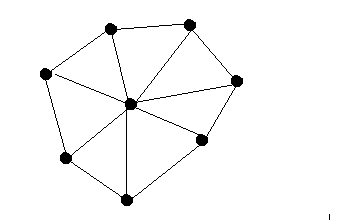
\includegraphics[scale=0.7]{img/10_2_20e_graph.png}
            \end{enumerate}
      \item[58.] Find the union of the given pair of simple
            graphs. (Assume edges with the same endpoints are the same.) \\
            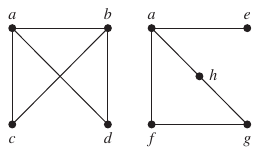
\includegraphics[]{img/10_2_58Q_graph.png}\\
            \answer \\
            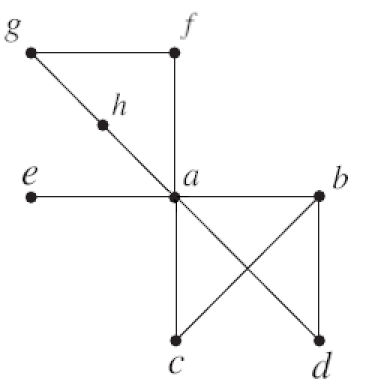
\includegraphics[scale = 0.65]{img/10_2_58A_graph.png}



\end{itemize}

\subsection{10.3}
%TODO: 10.3 – 2, 4, 6, 8, 12, 14, 26, 38, 42

\subsection{10.4}
%TODO: 10.4 – 2, 8, 14

\subsection{10.5}
%TODO: 10.5 – 2